\documentclass[12pt]{article}
 
\usepackage[margin=.75in]{geometry} 
\usepackage{amsmath,amsthm,amssymb}
\usepackage{bm}
\usepackage{enumitem}
\usepackage{color}
\usepackage{graphicx}
\usepackage{verbatim}
\setenumerate{listparindent=\parindent}
\definecolor{gray}{gray}{0.6}

\setenumerate{listparindent=\parindent}
 
\newcommand{\N}{\mathbb{N}}
\newcommand{\Z}{\mathbb{Z}}
\newcommand{\E}{\mathbb{E}}
\DeclareMathOperator*{\Cov}{Cov}
\DeclareMathOperator*{\Col}{Col}
 

\newcommand*{\thead}[1]{\multicolumn{1}{|c|}{\bfseries #1}}

\usepackage{listings}
\lstset{
language=R,
basicstyle=\scriptsize\ttfamily,
commentstyle=\ttfamily\color{gray},
%numbers=left,
numberstyle=\ttfamily\color{gray}\footnotesize,
stepnumber=1,
numbersep=5pt,
backgroundcolor=\color{white},
showspaces=false,
showstringspaces=false,
showtabs=false,
frame=single,
tabsize=2,
captionpos=b,
breaklines=true,
breakatwhitespace=false,
%title=\lstname,
escapeinside={},
keywordstyle={},
morekeywords={}
} 

%\usepackage{fancyhdr} % Required for custom headers 
%%\usepackage{lastpage} % Required to determine the last page for the footer
%
%\pagestyle{fancy}
%\lhead{Stat 151A (HW4)}
%\chead{Michael Knopf (24457981)}
%\rhead{April $13^\text{th}$, 2015}
%\lfoot{}
%\cfoot{}
%\rfoot{}
%%\rfoot{Page\ \thepage\ of\ \pageref{LastPage}}
%\renewcommand\headrulewidth{0.4pt}
%%\renewcommand\footrulewidth{0.4pt}


\begin{document}
\title{I'll Never Let Go, Jack \\ Stat 151A}
\author{Michael Knopf}
 
\maketitle

\begin{figure}[ht!]
\centering
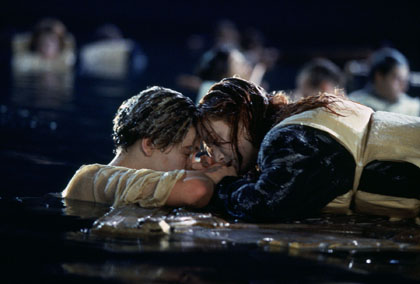
\includegraphics[width=100mm]{titanic_pic.jpg}
\end{figure}

\section{Introduction}

After performing an exhaustive search, I am frustrated that I have found neither Jack nor Rose in the Titanic dataset.  Clearly, there are missing observations.  I have refrained from adding 2 rows - one with $Survived = 1$ and the other with $Survived = 0$ - to reflect Jack and Rose in the data, since I would have to rewatch the entire movie to determine the other values for these observations.

From my initial intuition, I would expect $Age$, $Parch$, and $SibSp$ to be useful in prediction.  However, they may need to be transformed in order to be useful, and their interactions should be considered as well.  For instance, if a young child was on-board with a parent, it is likely that the parent would try to ensure the child's survival, even to the point of disregarding his or her own (unless they are a terrible parent).  However, a child on board without his or her parents might be at a disadvantage.

\pagebreak
\section{Data}
A description of the provided data is tabulated below.
\begin{center}
\renewcommand{\arraystretch}{1.2}
\begin{tabular}{|l|l|}
\hline
\thead{Variable} & \thead{Description} \\
\hline 
PassengerId & A unique ID for each passenger in the dataset \\
\hline 
Survived & 0: Died, 1: Survived \\
\hline 
Pclass & A proxy for passenger class, 1 being the highest class and 3 the lowest. \\
\hline 
SibSp & The sum total of the number of siblings or spouses aboard with the passenger \\
\hline 
Parch & The sum total of the number of parents or children aboard with the passenger \\
\hline 
Fare & Fare price \\
\hline 
Embarked & Port departed from: Cherbourg, Queenstown, Southhampton \\
\hline 
\end{tabular} 
\end{center}

The first issue with the data is missing values for $Age$.  Because $Age$ proved to be an important explanatory variable, I did not want to simply exlude it from the model.  One method of dealing with this that I considered was to first predict missing values of $Age$ from the other provided variables (excluding $Survived$), and then use the predicted values as substitutes in the main model.  However, this method would compound errors and increase multicolinearity.  Since there are a significant number of missing values (177 out of 891 in the training set, 86 outof 418 in the test set), this is not an acceptable solution.

The solution I decided on was to use two separate models: one including $Age$, and one not including it.  For the model including $Age$, I fit the response to the set of observations where $Age$ was recorded.  For the model without $Age$, I fit the response to the entire training set.

A second question that arose was whether certain continuous variables should be convereted to categorical.  In many models, the significance of $Parch$ was improved by transforming it to $(Parch == 0)$, and $Embarked$ was only useful when looked at as the variable $(Embarked == 'S')$.  However, in the model I ended up choosing, neither of these were useful.

The only change I ended up making was on the variable $Age$.  It turned out that the given continuous variable was less important than the categories ``child," ``young adult," and ``old adult."  The question of what age ranges define these categories was something I had to decide after inspecting several models, but the ranges that eventually proved most effective were $Age \leq 9$, $10 \leq Age \leq 36$, and $Age \geq 37$.

The last topic worth mentioning is interaction terms.  The only interaction that seemed worth using was that between the $Age$ categories and the $SibSp$ variable.  This interation term was significant in the model, however I chose not to use it because I was very concerned with overfitting.  With the amount of data present, I was more concerned with limiting model size at that point.

\begin{figure}[ht!]
\centering
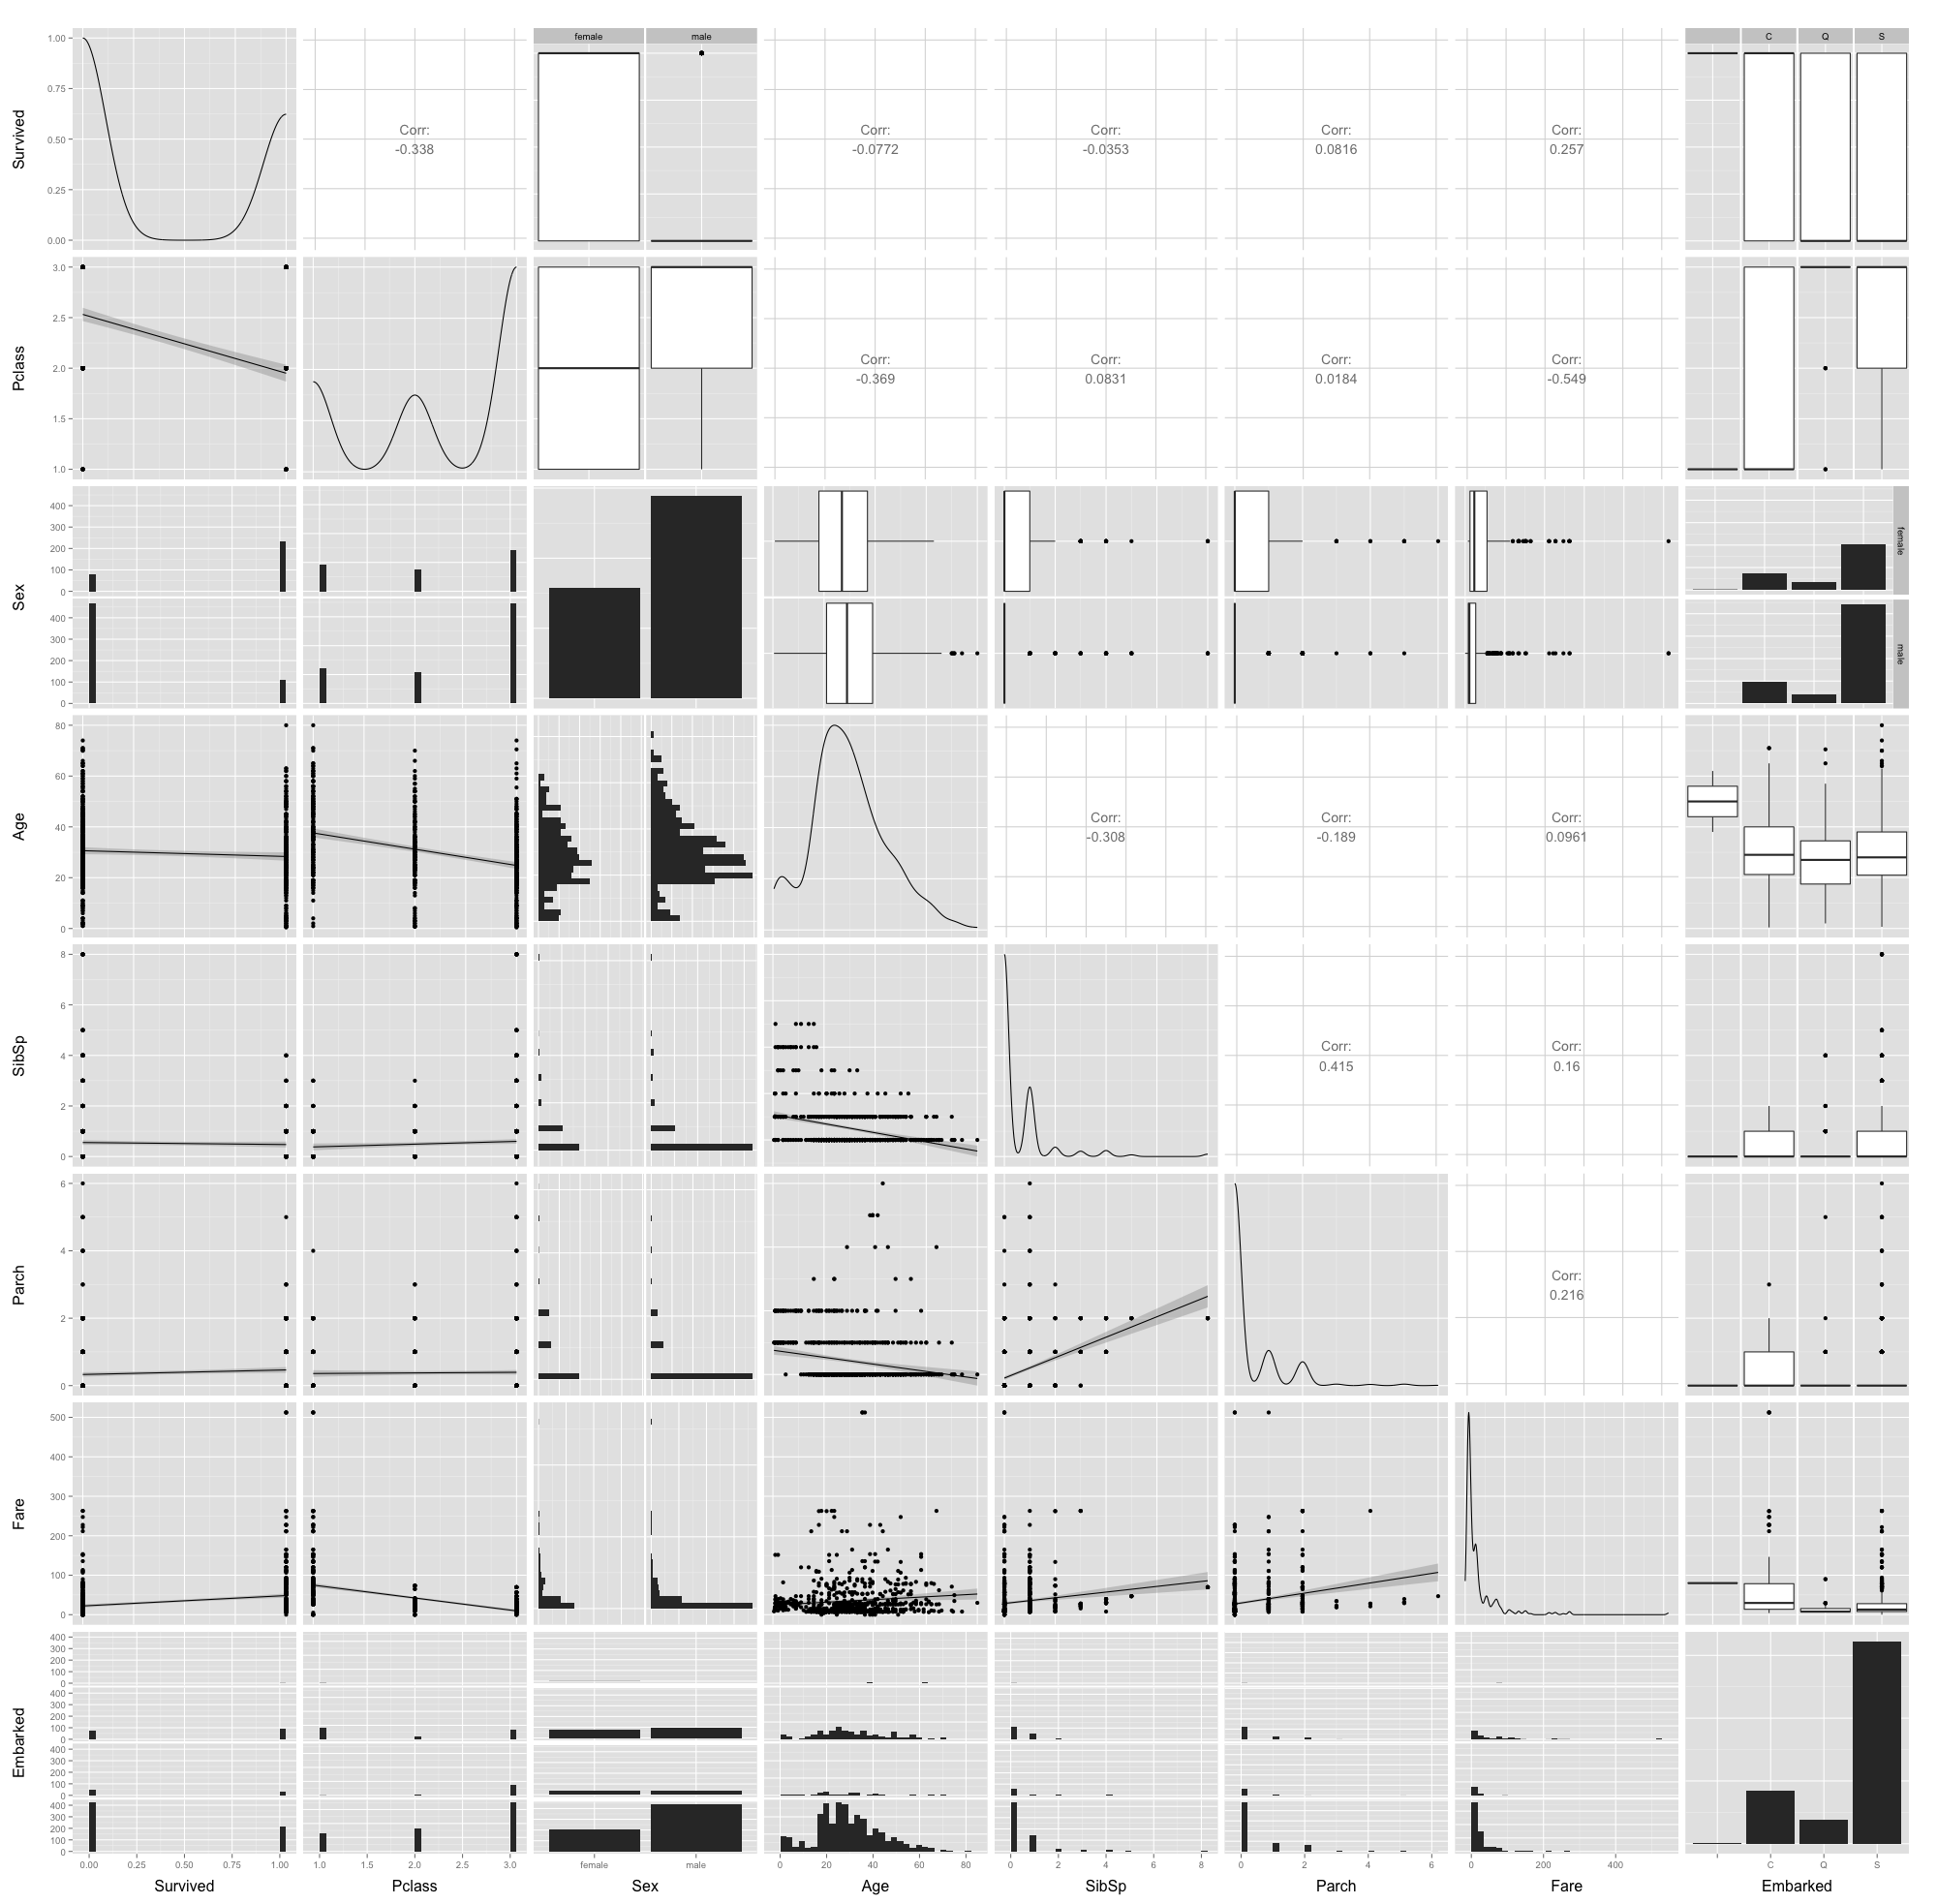
\includegraphics[width=180mm]{pairs.png}
\caption{Pairwise plots of all present variables.  Relationships between the variables used in the chosen models are minimal.}
\end{figure}
%\lstinputlisting{./interpretationcode.R}

\section{Variable Selection}



Due to the small number of explanatory variables, it is computationally possible to simply compare all possible models.  This simplified the analysis greatly.  I compared the $AIC$ for every possible model and found that the best scoring models (up to whether or not they include $Age$) were the two I had already suspected were the best fits ($Age.cat$ is the categorical variable described in section 2):

$$Survived = Pclass + Sex + Age.cat + SibSp$$
$$Survived = Pclass + Sex + SibSp$$

The way I originally found these models was by backward selection based on p-value, so I was satisfied that they had the best $AIC$ score as well.

Next, I used a confusion matrix to find the best threshold for prediction.  I went through a set of 1000 possible thresholds, looking for which produced the best results.  All such values were consecutive, so I took their mean as my final cutoff.  The thresholds I chose were $.52$ and $.62$, respectively.

After looking at many aspects of other candidate models, I finally performed 7-fold cross-validation on these models, as well as on all others possible, to evaluate their performance.  I used two methods: in one, I measured deviance to be the difference between the predicted probability of survival and the observed survival status; in the other, I simply looked at the number of incorrect predictions, where I predict based on whether the probability is above the threshold or not.  The statistics I took into account were
\begin{enumerate}
\item Sum of the deviances for each test set.
\item Variance of deviances across the test sets.
\end{enumerate}
Of course, we want the total deviance of the model to be low.  However, if the model's performance varies greatly between test sets, this is a problem as well.  The models I chose had the best score in the deviance category, and their scores were very low in the variance category.  Overall, they were the best performing models.  Summaries of the cross-validation are given below in Figure 2.

\begin{figure}[ht!]
\centering
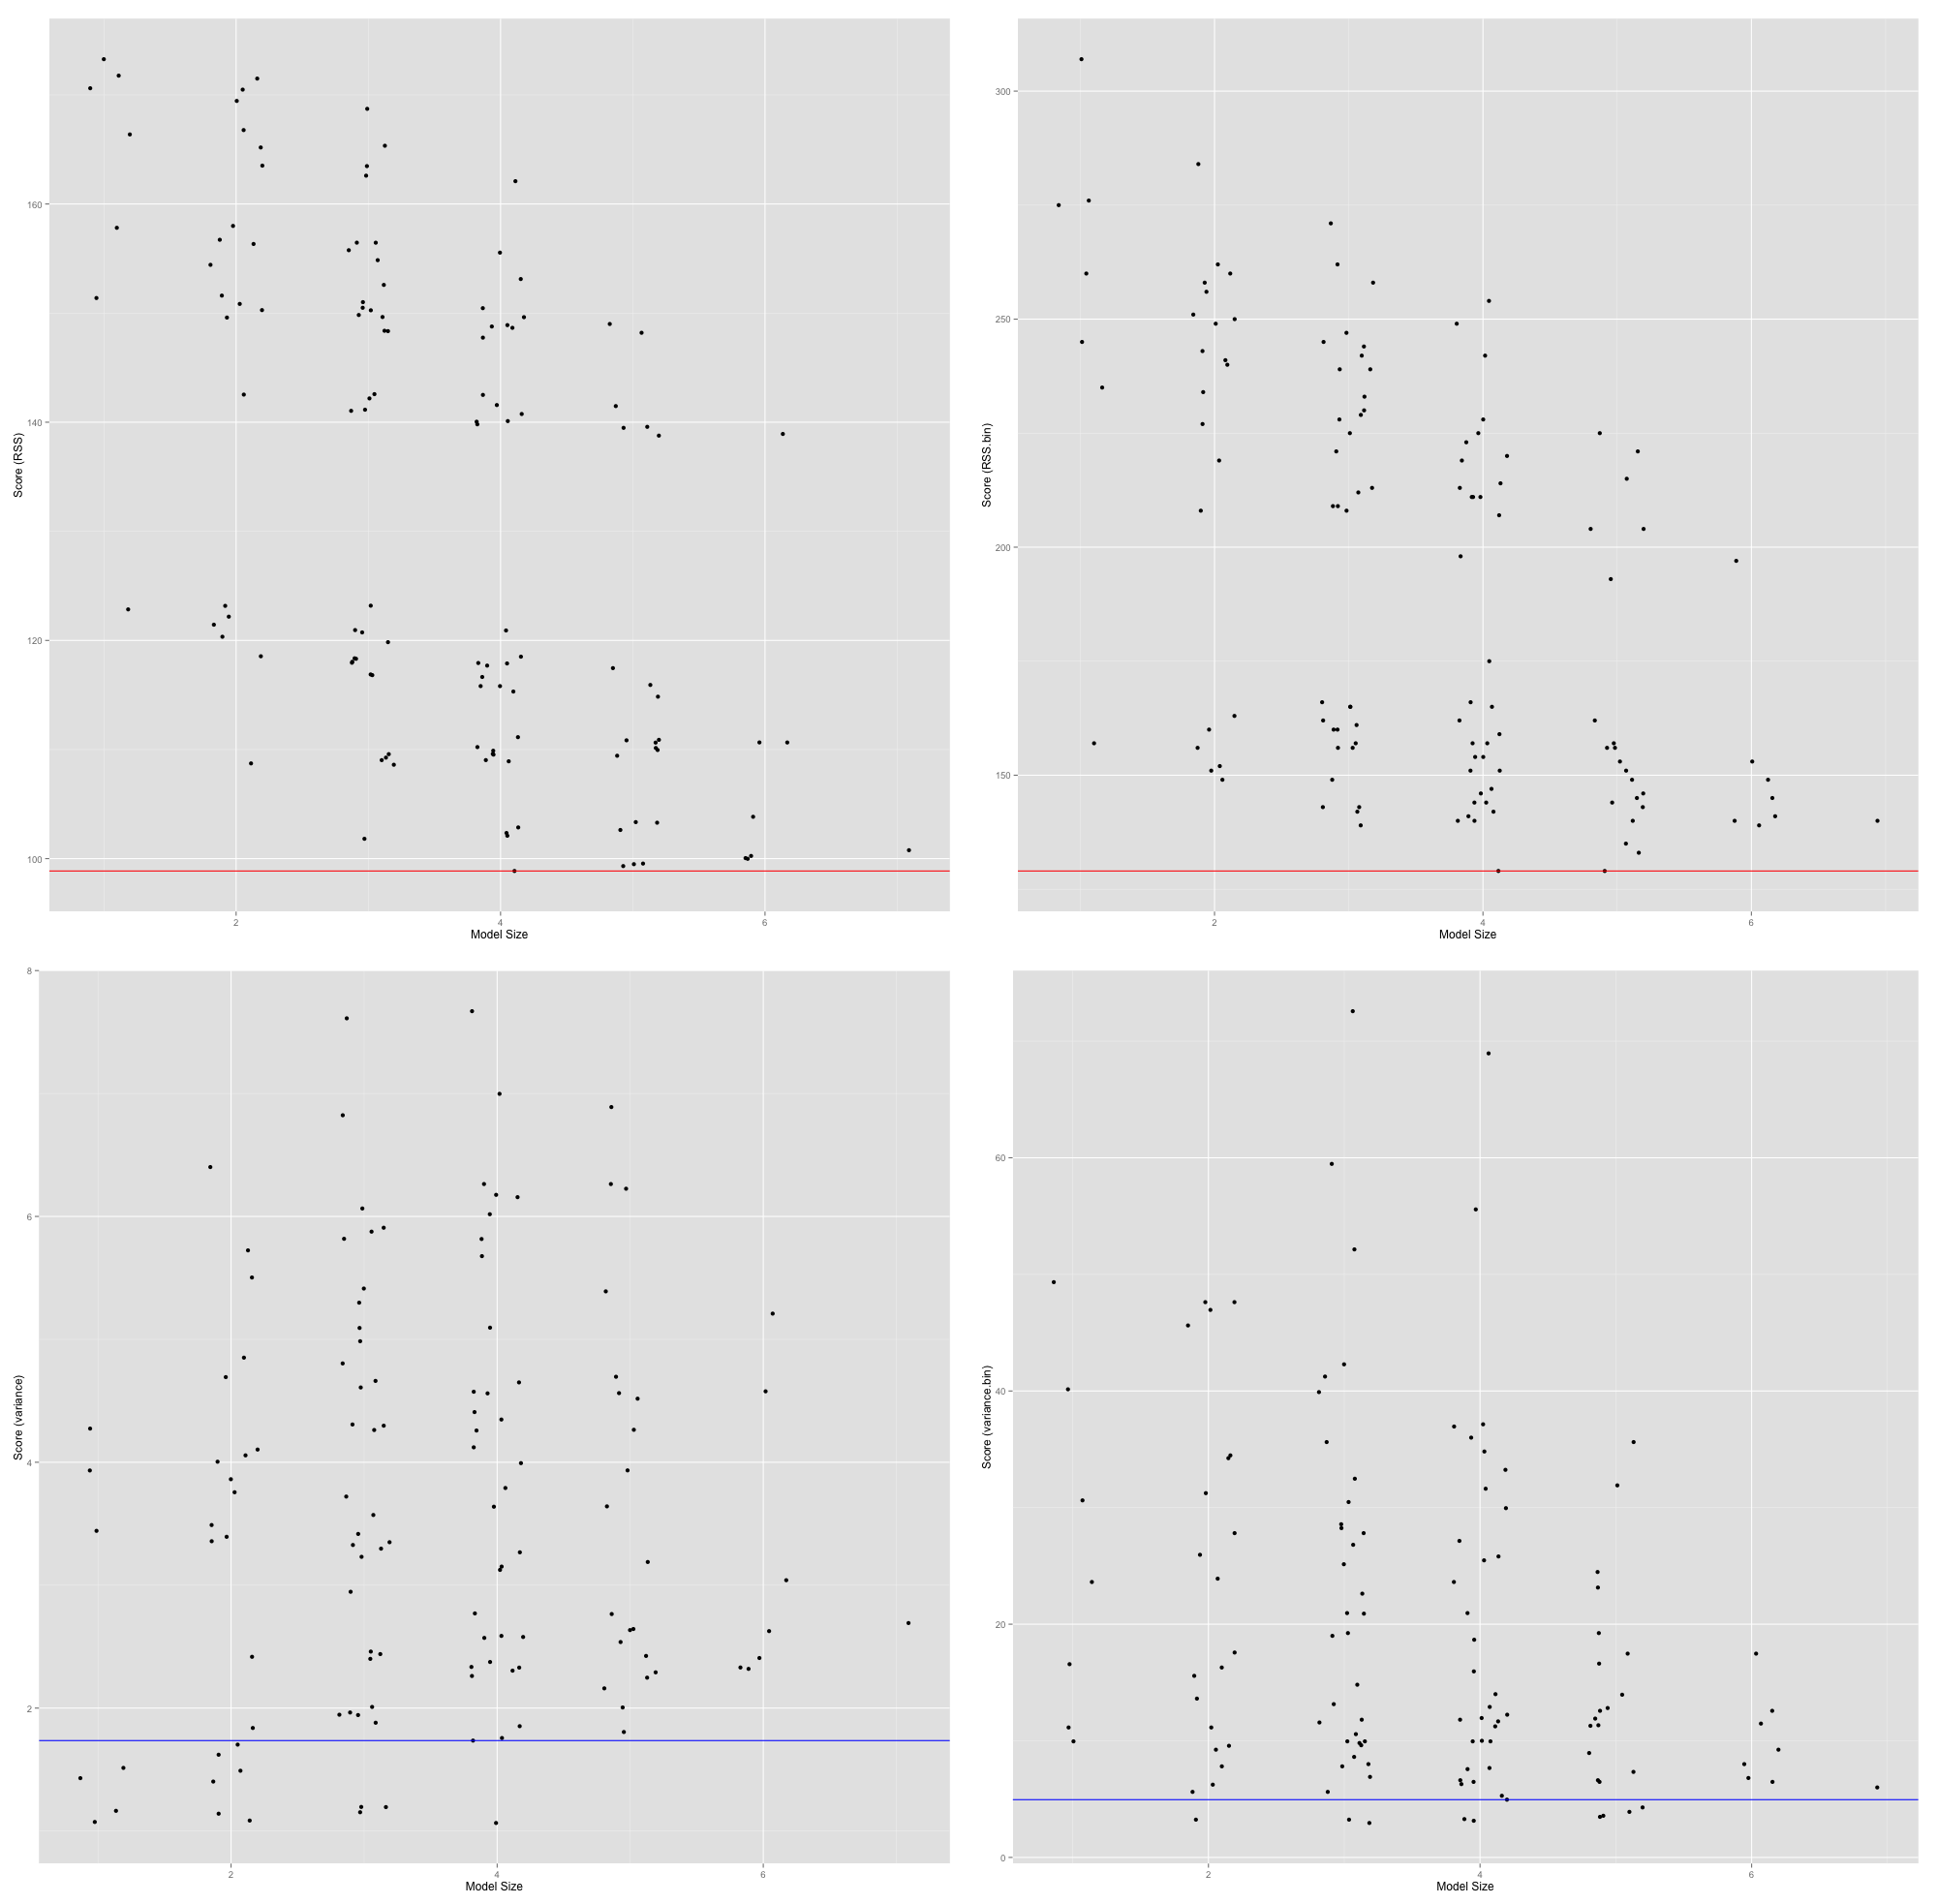
\includegraphics[width=180mm]{cv.png}
\caption{On the left are CV scores using predicted probabilities.  On the right are CV scores using pure predictions.  The top plots are total deviance against model size, the bottom are variance of deviances across the test sets against model size.  The lines mark the scores of the chosen model (including $Age$).}
\end{figure}

\section{Predictions}

Using the thresholds determined by confusion matrices, I predicted the value of $Survived$ for the test set observations.  For those which inclued $Age$, I used the first model.  For those that did not, I use the second.

Next, I used classification trees to predict these values as well.  I will not go into the methods I used to construct the trees, because it was not the main focus of my analysis.  However, the predictions only differed on 34 observations, and for the vast majority of these, the predicted probability of survival was very close to the threshold.  Also, whether or not $Age$ was present in these observations was insignificant, which is good (the proportion of observations without $Age$ was $.2057416$ in the test set $.2058824$ in the set of observations on which the two prediction methods disagreed).

In order to predict for these observations, I looked at them individually, adjusting the threshold and sometimes looking at how a model with one extra variable would predict their survival.  Ultimately, I split them into groups based on the glm predicted probability and made decisions for each group on a case-by-case basis, since there were not very many of them.

\noindent The prediction success rate was $0.77751$.

\pagebreak
\section{Code}
The following code is not commented well.  I did not have as much time to spend on this project as I did on the second midterm.  Many times, I went back and edited old code in order to reuse it.  Also, some variables have been instantiated or updated in one script, but are also being used in another.  Ultimately, the code worked perfectly for my purposes, but is no longer very readable.

\noindent First inspection of data:
\lstinputlisting{./data.R}
Second inspection of data:
\lstinputlisting{./trial2/data2.R}
Variable selection:
\lstinputlisting{./trial2/selection2.R}
Choosing thresholds with confusion matrices:
\lstinputlisting{./interpret.R}
Cross Validation:
\lstinputlisting{./trial2/crossvalidation2.R}
Predictions:
\lstinputlisting{./trial2/test.R}

\end{document}













